%!TEX root = ../document.tex

\section{Paper Prototype}
\label{sec:PAPER_PROTOTYPE}

After ideation we started prototyping to get user feedback on our ideas. 
We focused on the ideas regarding the editor enrichment in order to provide real data previews and performance feedback.
We decided to build an interactive paper prototype because of the simplicity of paper prototyping and the ability to test the usability of the overall design while manipulating the prototype via Post-its.
Since we aim to improve developer's productivity this usability testing is crucial for our idea. \\


\begin{figure}
\begin{centering}
    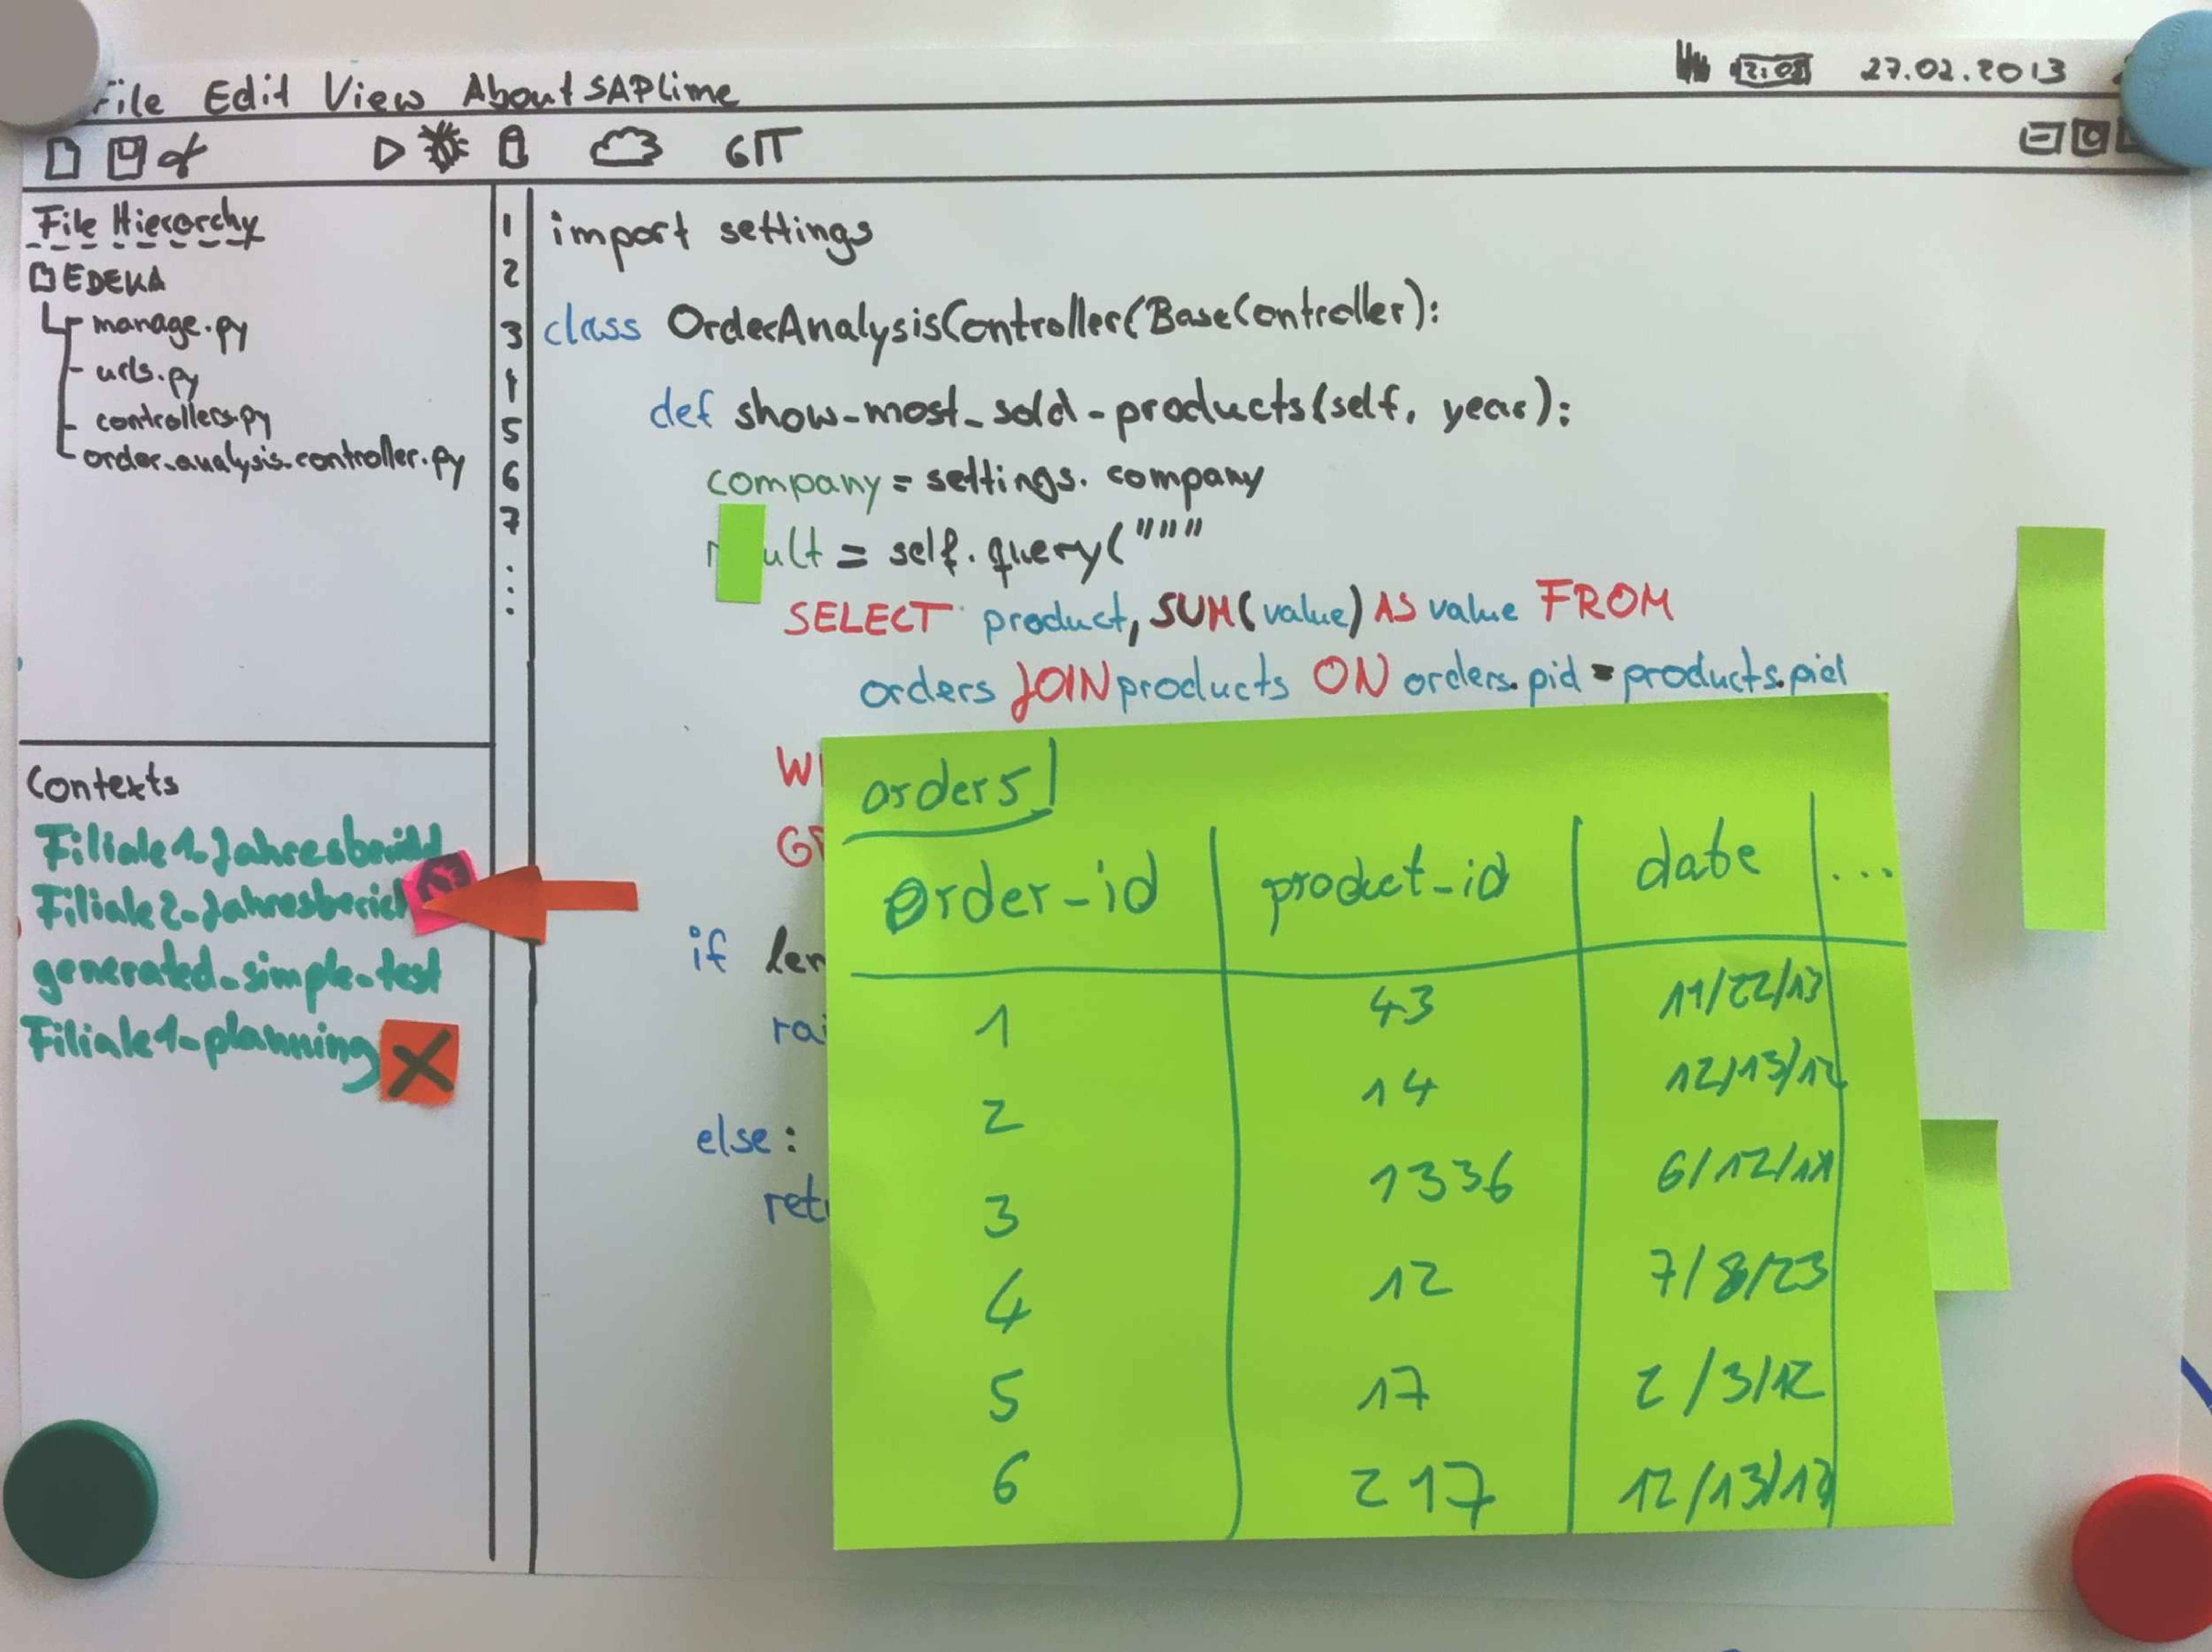
\includegraphics[width=1.0\linewidth]{images/paper_prototype2}
    \caption{Table Popup on our paper prototype after selecting the data table entity "orders"}
    % #selfrespect
    \label{fig:paper_prototype2}
\end{centering}
\end{figure}

We came up with an A3 cardboard that represents our conceived code editor. (Figure \ref{fig:paper_prototype2})
It shows a piece of code in a Python-like programming language with embedded SQL statements.
The editor benefits from global syntax highlighting and shows a new panel in the lower left.
This Panel includes a list of possible data contexts for this particular function.\\

For the user testing sessions we prepared several Post-its to simulate highlighting, cursor positioning and popup windows. 
As shown in Figure \ref{fig:paper_prototype2}, we used small, red paper squares to indicate either performance or functional problems in some of the data contexts. 
A small red arrow hints to the currently selected data context; the small green Post-it represents the cursor and can be moved by the user. 
The green stripes on the right mark the control flow that was covered by the execution of the currently selected data context. \\

When the user moves the cursor onto the identefier of a table used in the SQL query, a popup is presented that provides relevant information on this table.
Figure \ref{fig:paper_prototype2} shows an example of these Post-it-popups, when selecting the table "orders". 
For different tables and data contexts we prepared several Post-its with empty tables, too large tables and single rows that could be attached if the user wants to insert a row.\\

For our testing scenario we marked one of the contexts as erroneous and another as a performance bottleneck. 
The tested person was intended to inspect the several tables and examine the performance bottleneck or the program error respectively.







